\section{Choice of a Sparse Direct Solver Library}
\label{subseq:mm-library-choice}

% NOTE:
% all equation starts with prefix: lc, for this section


Fair to say, there is no single algorithm or software that is best for all types of linear systems \cite{list-of-sparse-direct-solvers}. Nowadays there exist many different sparse direct solvers on the market. Some of them are tunned for specific linear systems i.e. symmetric positive definite, systems with symmetric sparsity pattern, system with complex numbers, etc., some are targeted for the most general cases. Some packages can handle data parallelism in different ways even within the same library depending on the system size and other criteria. Hence, parallel performance highly depends on a specific implementation of a method. Table \ref{table:mm-library-spec} displays a short summary of almost all available and well-known packages, at the time of writing, in this field based on works \cite{list-of-sparse-direct-solvers} and \cite{petsc-web-page}.\\


\todo{add footnotes of Open*}

\begin{table}[ht]
\centering
\begin{tabular}{|c|c|c|c|c|}
\hline
Package & Method             & Matrix Types                 & PETSc Interface & License      \\ \hline
Clique       & Multifrontal       & Symmetric      & Not officially  & Open  \\ \hline
MF2          & Multifrontal       & Symmetric pattern & No              & -            \\ \hline
DSCPACK      & Multifrontal       & SPD                          & No              & Open* \\ \hline
MUMPS        & Multifrontal       & General                      & Yes             & Open  \\ \hline
PaStiX       & Left looking & General                      & Yes             & Open  \\ \hline
PSPASES      & Multifrontal       & SPD                          & No              & Open* \\ \hline
SPOOLES      & Left-looking       & Symmetric pattern & No              & Open* \\ \hline
SuperLU\_DIST & Right-looking      & General                      & Yes             & Open  \\ \hline
symPACK      & Left-Right looking & SPD                          & No              & Open  \\ \hline
S+           & Right-lookin       & General                      & No              & -            \\ \hline

PARDISO         & Multifrontal       & General                      & No              & Commercial   \\ \hline

WSMP         & Multifrontal       & General                      & No              & Commercial   \\ \hline
\end{tabular}
\caption{List of packages to solve sparse linear systems using direct methods on distributed memory parallel machines \cite{list-of-sparse-direct-solvers}, \cite{petsc-web-page}}
\label{table:mm-library-spec}
\end{table}


We only listed libraries that can run on distributed memory parallel machines. Almost all of them also support shared memory environment in some degree. Nonetheless there also exist libraries that  run either only sequentially (UMFPACK, SPARSE, TAUCS, SuperLU) or only on shared memory machines (PanelLLT, SuperLU\_MT).\\


% the most important aspect that we want to compare and consider is how numerical pivoting has been implemented for all chosen libraries. Numerical pivoting is [wiki]. Numerical pivoting in run time can lead to lots of problems


% to the end: we can see that MUMPS gives us better functionality. We can  explicitly control numerical pivoting and thus storage requirements, load balance and numerical accuracy 

We can see, from table \ref{table:mm-library-spec}, that only MUMPS, PaStiX and SuperLU\_DIST cover all our initial requirements: open-source license and direct interface to the PETSc library. However, these libraries implement different sparse direct methods, namely: multifrontal, left-looking and right-locking, respectively. Moreover, they handle partial pivoting in different ways.\\


It is known that partial pivoting is necessary to achieve a good numerical accuracy during Gaussian Elimination. It interchanges rows and columns of a matrix in such a way to avoid small numerical values along the diagonal. In case of sparse direct solvers, the numerical pivoting, in run-time, usually distorts all predictions that have been made during the analysis phase and can lead to significant fill-in and load unbalanced, with respect to floating-point operations, during factorization. Hence, implementation of numerical pivoting, especially during parallel execution, plays the most important role in performance for this group of methods.\\


Both PaStiX and SuperLU\_DIST libraries use so-called static pivoting where the pivot order is chosen before numerical factorization and kept fixed during factorization.\\


The main advantage of static pivoting is that it allows to better optimize the data layout, load balance, and communication scheduling \cite{superlu-manual}. However, it leads to a higher risk of numeric instability. Therefore, both PaStiX and SuperLU\_DIST provide a few ways to perform the solution refinement.\\


For instance, SuperLU\_DIST uses diagonal scaling, setting very tiny pivots to larger values, and iterative refinement (listing \ref{lst:iterative-refinement}). While PaStiX allows the user to choose a refinement strategy between GMRES, CG (for SPD systems) and iterative refinement as well. At this point it is interesting to notice that we came to the same conclusion as the PasTiX developers with respect to the solution refinement using Krylov iterative methods.\\


Iterative refinement, shown in listing \ref{lst:iterative-refinement}, is claimed to converge to a \todo{can we use decent here?} decent precision within 2 or 3 steps in work \cite{mm-backward-error}. However, in practice, we noticed that the iterative refinement can work not as expected, especially in case of lowered partial pivoting constrains.\\

For completeness, we have to mention that the variable $too\_large$ is, in fact, an estimation of the backward error \cite{mm-backward-error} which can be expressed as following:

\begin{equation}
\frac{|b - A\hat{x}|_{i}}{(|b| + |A| |\hat{x}|)_{i}}
\end{equation}

where $\hat{x}$ is the computed solution and $|\bullet|$ is the element-wise module operation.\\

 
\begin{minipage}{\linewidth}

\begin{lstlisting}[language=python, caption={A simple iterative refinement}, frame=single, label={lst:iterative-refinement}]
# perform analysis and numerical factorization 
# phases
LU = SparseDirectSolver(matrix=A)

# compute initial solution
x = Solve(factorization=LU, rhs=b)

# compute initial residual
r = A * x - b

while r > too_large:
	# find correction
	d = Solve(factorization=LU, rhs=r)
	
	# update solution
	x = x - d
	
	# update residual
	r = A * x - b
\end{lstlisting}
\end{minipage}
\todo{listing of iterative refinement}

% Drawback static pivoting is implicit wrt memory consumtion

In contrast to PaStiX and SuperLU\_DIST, MUMPS performs partial pivoting in run-time during the numerical factorization phase. To limit the amount of numerical pivoting, and stick better to the
sparsity predictions done during the symbolic factorization, partial pivoting can be relaxed, leading to the partial threshold pivoting strategy \cite{mumps-manual}.\\

A pivot $|a_{i,i}|$ is accepted if it satisfies:\\
\begin{equation}\label{eq:lc-1}
|a_{i,i}| \geq u \times max_{k=i \cdots n} |a_{k,j}|
\end{equation}

where $u$ is value between 0 and 1.\\

To improve solution accuracy, MUMPS, as PasTiX and SuperLU\_DIST, provides the iterative refinement as a post-processing step as well.\\


The most important feature which MUMPS introduces is so-called delayed pivots. It can happen that equation \ref{eq:lc-1} cannot be satisfied within a fully-summed block of a frontal matrix (equation  \ref{eq:mm-10}) and we also cannot consider elements outside the block since the corresponding rows are not fully-summed. In this case, some rows and columns will remain unfactored, or delayed, in the front. They are going to be sent the frontal matrix of the parent, as part of the contribution block and the process will repeat. The delayed pivot approach helps to improve numerical accuracy, however, it causes additional fill-in in the parent node.\\


In spite of obvious complexity of dynamic partial pivoting, MUMPS allows the user to explicitly control run-time behavior of the algorithm due to partial threshold pivoting strategy. This provides an opportunity for optimization and tuning in some degree.\\


PETSc (version 3.10) provides the full interface to both SuperLU\_DIST and MUMPS, whereas the interface to the PasTiX library is quite limited. In fact, in case of PasTiX, the user can only control the number of threads per MPI process and a level of verbosity, which makes this library to be less interesting for our subsequent (following) research.\\


In order to evaluate the overall parallel performance of the libraries, we performed a few flat-MPI tests with the GRS matrix using the HW1 machine. Before testing, we downloaded and configured the libraries, MUMPS version 5.1.2, PasTiX version 6.0.0, SuperLU\_DIST version 5.4, within the PETSc environment with their \textbf{default settings}. As a profiling tool, we used the internal PETSc profiler. A time limit of 15 minutes was set up for each test case to prevent blocking of a compute node in case if out-of-core execution. Results of the tests are summarized in tables \ref{table:lc-cube-5-result}, \ref{table:lc-cube-64-result}, \ref{table:lc-k3-18-result} and in appendix \ref{app:app-lc}. Numerical values in tables are given in \textbf{seconds}.\\


\begin{table}[ht]
\centering
\begin{tabular}{|c|c|c|c|l|c|c|c|c|}
\cline{1-4} \cline{6-9}
MPI & MUMPS    & PaStiX   & SuperLU  &  & MPI & MUMPS    & PaStiX   & SuperLU  \\ \cline{1-4} \cline{6-9} 
1   & 7.02E-02 & 8.72E-02 & 3.17E+00 &  & 11  & 7.55E-02 & 8.89E-02 & 5.82E-01 \\ \cline{1-4} \cline{6-9} 
2   & 6.73E-02 & 7.10E-02 & 1.43E+00 &  & 12  & 7.61E-02 & 1.06E-01 & 4.37E-01 \\ \cline{1-4} \cline{6-9} 
3   & 6.36E-02 & 7.01E-02 & 1.07E+00 &  & 13  & 7.84E-02 & 9.72E-02 & 5.43E-01 \\ \cline{1-4} \cline{6-9} 
4   & 6.28E-02 & 7.11E-02 & 8.17E-01 &  & 14  & 8.06E-02 & 1.02E-01 & 4.22E-01 \\ \cline{1-4} \cline{6-9} 
5   & 6.50E-02 & 7.15E-02 & 7.51E-01 &  & 15  & 8.20E-02 & 1.19E-01 & 3.91E-01 \\ \cline{1-4} \cline{6-9} 
6   & 6.72E-02 & 7.62E-02 & 6.15E-01 &  & 16  & 8.07E-02 & 1.19E-01 & 4.44E-01 \\ \cline{1-4} \cline{6-9} 
7   & 6.91E-02 & 7.69E-02 & 6.48E-01 &  & 17  & 8.38E-02 & 1.22E-01 & 5.19E-01 \\ \cline{1-4} \cline{6-9} 
8   & 6.89E-02 & 8.17E-02 & 5.41E-01 &  & 18  & 8.40E-02 & 1.26E-01 & 3.77E-01 \\ \cline{1-4} \cline{6-9} 
9   & 7.50E-02 & 8.28E-02 & 5.02E-01 &  & 19  & 8.58E-02 & 1.33E-01 & 5.47E-01 \\ \cline{1-4} \cline{6-9} 
10  & 7.22E-02 & 8.52E-02 & 4.64E-01 &  & 20  & 8.64E-02 & 1.49E-01 & 3.39E-01 \\ \cline{1-4} \cline{6-9} 
\end{tabular}
\caption{Results of a flat-MPI test of MUMPS, PasTiX and SuperLU\_DIST libraries with their default settings and the matrix \textbf{cube-5} (9352 equations)}
\label{table:lc-cube-5-result}
\end{table}


\begin{table}[ht]
\centering
\begin{tabular}{|c|c|c|c|l|c|c|c|c|}
\cline{1-4} \cline{6-9}
MPI & MUMPS    & PaStiX   & SuperLU  &  & MPI & MUMPS    & PaStiX   & SuperLU  \\ \cline{1-4} \cline{6-9} 
1   & 1.36E+00 & 1.39E+00 & time-out &  & 11  & 7.75E-01 & 8.15E-01 & time-out \\ \cline{1-4} \cline{6-9} 
2   & 1.00E+00 & 9.82E-01 & time-out &  & 12  & 7.81E-01 & 8.10E-01 & time-out \\ \cline{1-4} \cline{6-9} 
3   & 8.83E-01 & 1.06E+00 & time-out &  & 13  & 7.85E-01 & 8.35E-01 & time-out \\ \cline{1-4} \cline{6-9} 
4   & 8.17E-01 & 8.74E-01 & time-out &  & 14  & 7.85E-01 & 8.18E-01 & time-out \\ \cline{1-4} \cline{6-9} 
5   & 7.85E-01 & 8.50E-01 & time-out &  & 15  & 7.88E-01 & 8.46E-01 & time-out \\ \cline{1-4} \cline{6-9} 
6   & 8.06E-01 & 8.52E-01 & time-out &  & 16  & 7.81E-01 & 8.23E-01 & time-out \\ \cline{1-4} \cline{6-9} 
7   & 7.71E-01 & 8.33E-01 & time-out &  & 17  & 6.83E-01 & 8.49E-01 & time-out \\ \cline{1-4} \cline{6-9} 
8   & 7.66E-01 & 8.33E-01 & time-out &  & 18  & 7.96E-01 & 8.44E-01 & time-out \\ \cline{1-4} \cline{6-9} 
9   & 7.93E-01 & 8.35E-01 & time-out &  & 19  & 8.04E-01 & 8.65E-01 & time-out \\ \cline{1-4} \cline{6-9} 
10  & 8.07E-01 & 8.15E-01 & time-out &  & 20  & 6.85E-01 & 8.87E-01 & time-out \\ \cline{1-4} \cline{6-9} 
\end{tabular}
\caption{Results of a flat-MPI test of MUMPS, PasTiX and SuperLU\_DIST libraries with their default settings and the matrix \textbf{cube-64} (100657 equations)}
\label{table:lc-cube-64-result}
\end{table}


\begin{table}[h!]
\centering
\begin{tabular}{|c|c|c|c|l|c|c|c|c|}
\cline{1-4} \cline{6-9}
MPI & MUMPS    & PaStiX   & SuperLU &  & MPI & MUMPS    & PaStiX   & SuperLU \\ \cline{1-4} \cline{6-9} 
1   & 1.55E+02 & 6.44E+01 & crashed &  & 11  & 1.77E+01 & 3.81E+01 & crashed \\ \cline{1-4} \cline{6-9} 
2   & 6.28E+01 & 4.84E+01 & crashed &  & 12  & 1.60E+01 & 3.75E+01 & crashed \\ \cline{1-4} \cline{6-9} 
3   & 5.06E+01 & 5.02E+01 & crashed &  & 13  & 1.42E+01 & 3.58E+01 & crashed \\ \cline{1-4} \cline{6-9} 
4   & 4.17E+01 & 4.50E+01 & crashed &  & 14  & 1.45E+01 & 3.59E+01 & crashed \\ \cline{1-4} \cline{6-9} 
5   & 2.52E+01 & 3.98E+01 & crashed &  & 15  & 1.47E+01 & 3.57E+01 & crashed \\ \cline{1-4} \cline{6-9} 
6   & 2.58E+01 & 4.29E+01 & crashed &  & 16  & 1.41E+01 & 3.52E+01 & crashed \\ \cline{1-4} \cline{6-9} 
7   & 2.65E+01 & 4.30E+01 & crashed &  & 17  & 1.54E+01 & 3.45E+01 & crashed \\ \cline{1-4} \cline{6-9} 
8   & 2.59E+01 & 3.73E+01 & crashed &  & 18  & 1.52E+01 & 3.31E+01 & crashed \\ \cline{1-4} \cline{6-9} 
9   & 1.95E+01 & 4.08E+01 & crashed &  & 19  & 1.52E+01 & 3.31E+01 & crashed \\ \cline{1-4} \cline{6-9} 
10  & 1.91E+01 & 3.81E+01 & crashed &  & 20  & 1.38E+01 & 3.16E+01 & crashed \\ \cline{1-4} \cline{6-9} 
\end{tabular}
\caption{Results of a flat-MPI test of MUMPS, PasTiX and SuperLU\_DIST libraries with their default settings and the matrix \textbf{k3-18} (1155955 equations)}
\label{table:lc-k3-18-result}
\end{table}



We ran into a few problems with the SuperLU\_DIST library during the tests. Firstly, factorization exceeded the set time limit in case of \textbf{cube-64} and \textbf{k3-2} matrices. Secondly, we noticed the library crashed during processing of \textbf{k3-18}, \textbf{cube-645} and (partially) \textbf{pwr-3d} matrices. A debugging process showed that a segmentation fault occurred in \textit{pdgstrf} function during the numerical factorization phase. We still keep working on this problem together with the PETSc team in order to find a solution. \\

% FOR PRESENTATION: it can be due to wrong matrix representation in binary PETSc files. I ran into the same problem with METIS when it spinned the CPU for hours due to wrong CRS format


To complete and perform a fair comparison, an additional flat-MPI test was conducted with a 5-point stencil Poisson matrix with 100000 equations. We think this test can partially allow us to estimate parallel performance of systems like \textbf{k3-18}, \textbf{cube-645} where SuperLU\_DIST crashed. The results of the test are given in figure \ref{fig:5-point-stencil-solvers-comparison}.\\

\figpointer{\ref{fig:5-point-stencil-solvers-comparison}}
\begin{figure}[htpb]
  \centering
  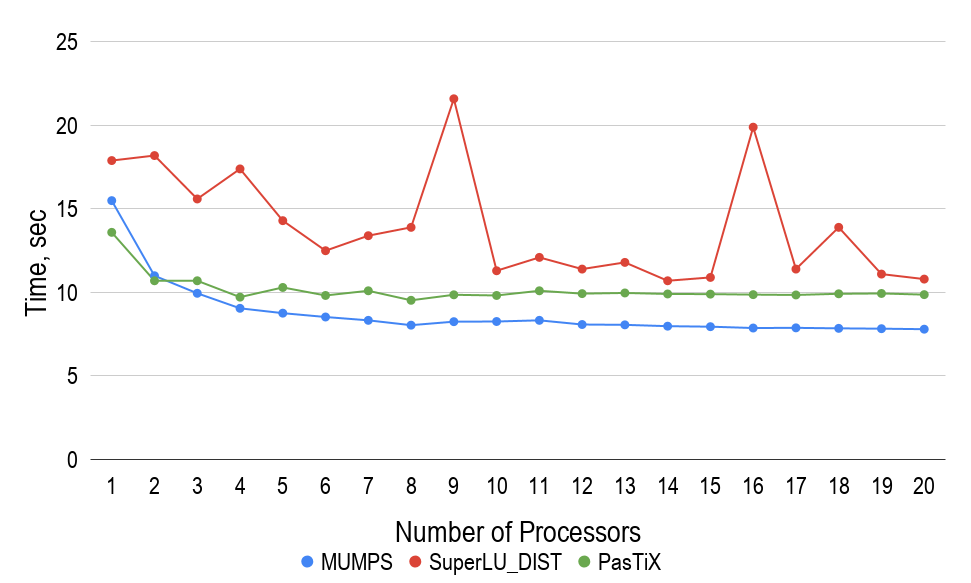
\includegraphics[width=0.85\textwidth]{figures/chapter-2/solvers-comparison-5-point-stencil.png}
\caption{Results of a flat-MPI test of MUMPS, PasTiX and SuperLU\_DIST libraries with their default settings and a 5 point-stencil Poisson matrix (1000000  equations)}
\label{fig:5-point-stencil-solvers-comparison}
\end{figure}

% FOR PRESENTATION: we think that 


According to the test results, it is clear that MUMPS significantly outperforms both SuperLU\_DIST and PaStiX. A literature review showed that \citeauthor{wsmp}, in paper \cite{wsmp}, came to nearly the same results comparing parallel performance of WSMP, MUMPS and SuperLU\_DIST libraries with respect to execution time for their matrix set. However, paper \cite{mm-comparison-of-packages} showed an almost opposite outcome. According to \citeauthor{mm-comparison-of-packages}, SuperLU\_DIST spent less time on factorization and solution phases, which almost always determines the total execution time, and, even more interesting, it scaled much better overall. We must note that both research groups used different machines and matrix sets. This fact actually seconds our idea that a choice of a suitable library can depend heavily on data and hardware.\\


Taking into consideration the results of our primary flat-MPI tests, the MUMPS library was chosen as a sparse direct solver for our hybrid approach and the following study. Furthermore, an overview of the MUMPS documentation also showed some room for performance tuning that we were going to discuss in detail in sections [bla], [bla] and  [bla].\\


However, it should be mentioned that we cannot exclude that SuperLU\_DIST  and PaStiX can perform similar, or even better, as the MUMPS library with appropriate parameters tuning or for another matrix set.\\
